\chapter{Discussion}\label{ch7:discuss}
\label{ch7:discussion}

Risk acts as a significant barrier to the adoption of geothermal energy as part of a larger energy portfolio for commercial oil \& gas companies. Here, the word \textit{risk} refers to the "potential inability to achieve overall program objectives within defined constraints" and can be characterized by a probability of occurrence and consequence of failure \citep{malone_development_2004}.  Companies considering investments in geothermal want to minimize risk exposure, so strategies to mitigate this risk will naturally act as enablers for investment in geothermal during the on-going energy transition.

Measure of the potential inability to achieve overall program objectives within
defined constraints and has two components: 1) the probability/likelihood of failing
to achieve a particular outcome, and 2) the consequence/impact of failing to achieve
that outcome

\section{Field Lifecycle}
\label{ch7:field_lifecycle}

Maturing a geothermal asset from initial concept through site decommissioning represents a complex project lifecycle spanning up to several decades in length. Figure \ref{fig:geothermal_field_lifecycle} illustrates the decomposition of a geothermal field lifecycle into a level 1 process flow that mimics that of a typical hydrocarbon field. The level 2 decomposition describes a work breakdown structure, each step with its own inherent risks. Here, the primary play risk elements for geothermal introduced in Section \ref{ch2:sysfund} have been reframed as four components: heat, permeability, fluids, and seal. Each appear in both the Exploration and Appraisal phases of the project. 

\begin{figure}
\centering
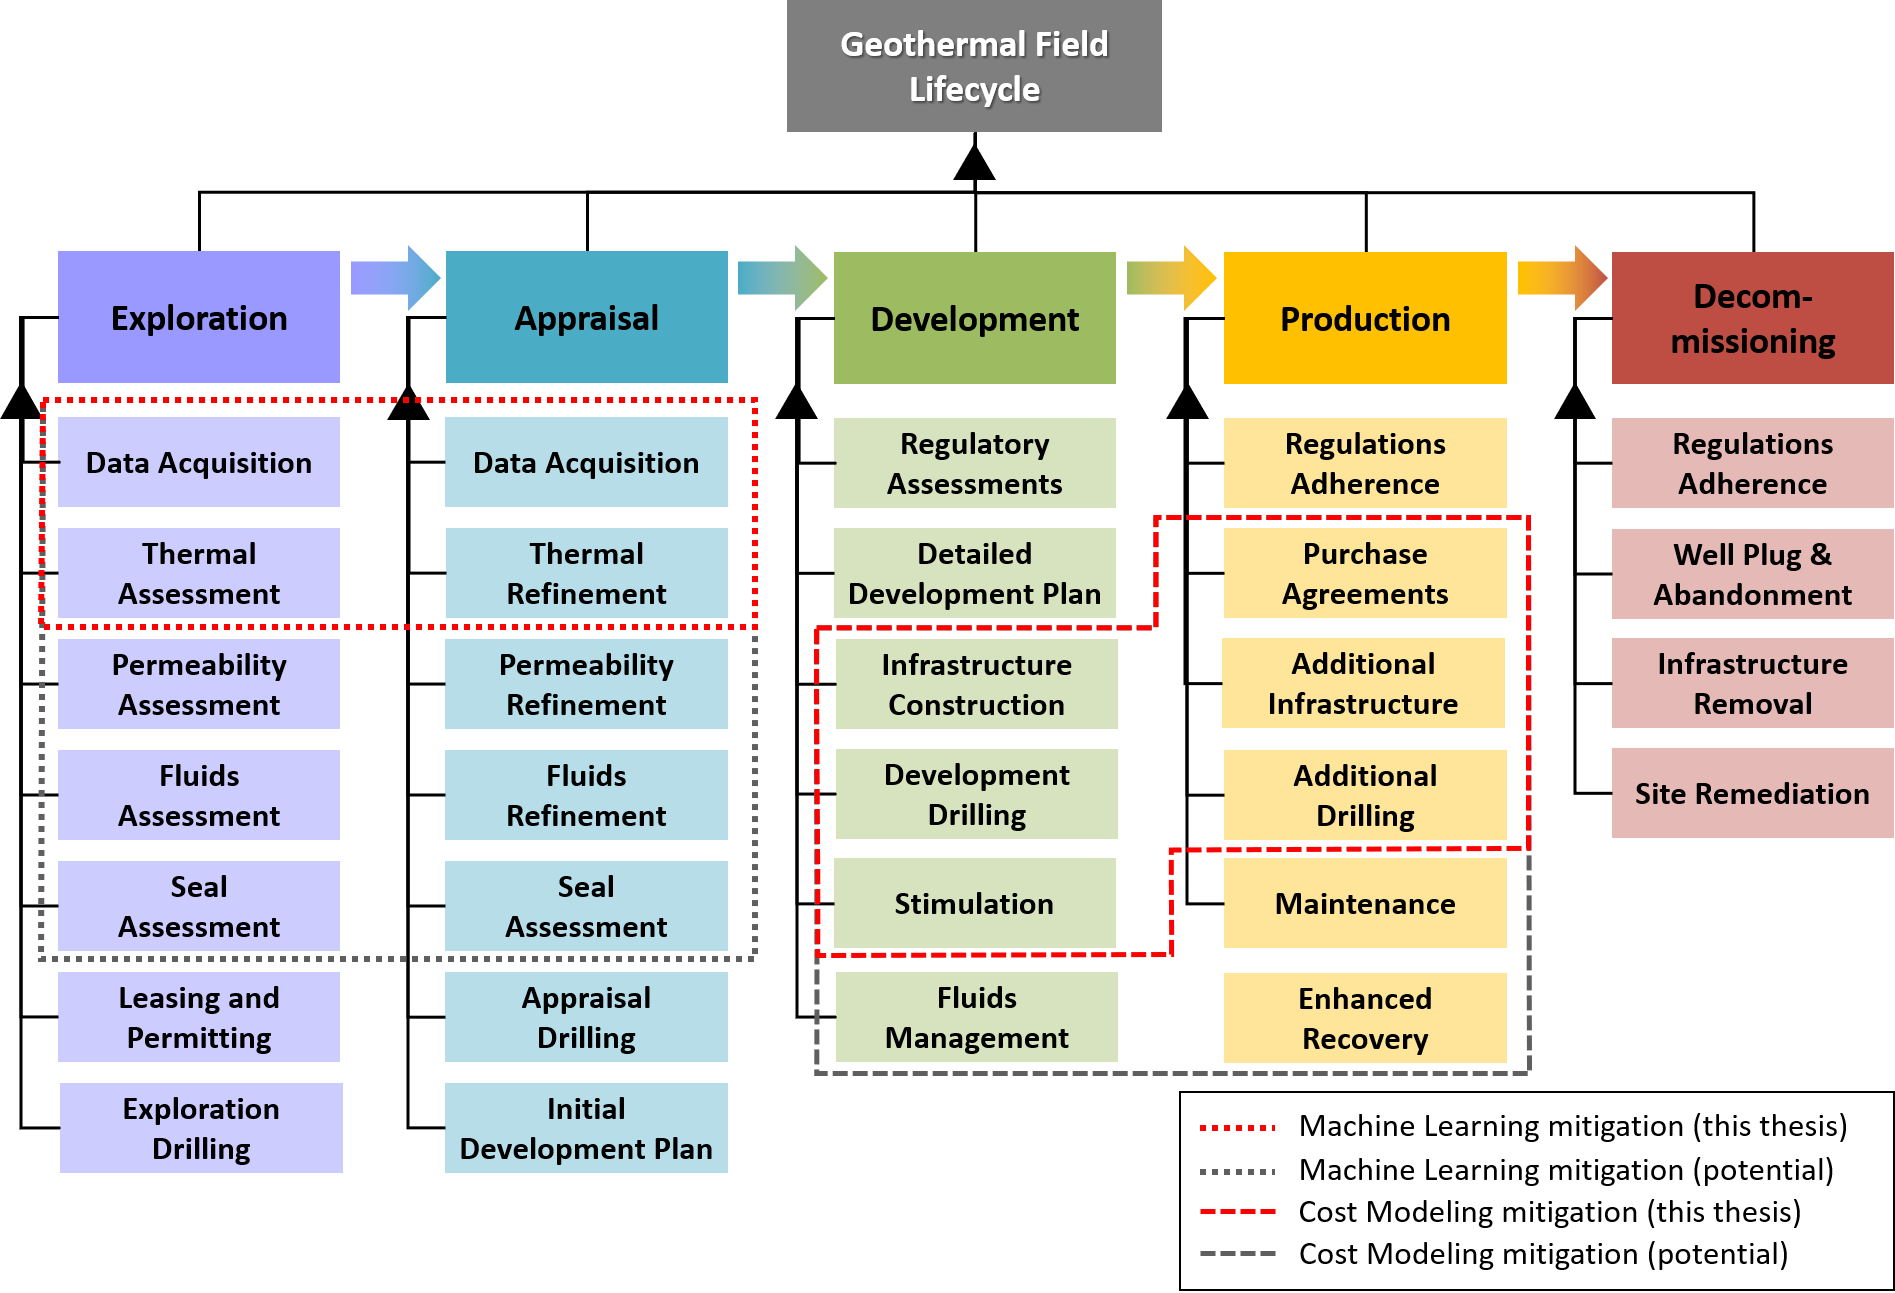
\includegraphics[width=\textwidth]{templates/images/Figure-SystemDecomposition.png}
\caption[Geothermal field lifecycle]{Proposed geothermal field lifecycle and two levels of decomposition defining major project phases and a high-level WBS. Dotted lines indicate where machine learning methods could mitigate risk in exploration and appraisal. Dashed lines depict where cost models might mitigate risk during the development and production phases.}
\label{fig:geothermal_field_lifecycle}
\end{figure}

The red dotted outline in Figure \ref{fig:geothermal_field_lifecycle} illustrates activities in the Exploration and Appraisal stages where machine learning methods described in Chapters \ref{ch3:expl_prep} and \ref{ch5:expl_ml} can reduce the overall risk profile. Geothermal exploration commonly focuses on areas where data and known resources are already present. Reviewing available data to identify feature relationships suggestive of favorable locations is an early pre-screening activity for mitigating the risk of costly exploration failures \citep{doughty_geovision_2018}. ML algorithms described in Chapter \ref{ch5:expl_ml} provide data-driven methods for uncovering these complex feature relationships and generating resource favorability maps rapidly and at low cost. Furthermore, feature importances derived from recursive feature elimination (Section \ref{ch5:logreg_rfe}), impurity measures like Gini index or entropy (Section \ref{ch5:impurity}), or Shapley analysis (Section \ref{ch5:xgb_shapley}) directly rank different data sources by their value for predictive modeling. These measures could also be used to guide exploration and appraisal spending on additional data purchases or acquisition efforts. For example, recognizing that silica geothermometer temperatures, heat flow measurements, crustal thickness, and density of volcanic dikes and springs all highly influence the geothermal gradient classification model (see Section \ref{ch5:xgb_shapley}), an exploration team could focus time and budget on 1) field surveys for silica concentration sampling, 2) field or remote-sensing mapping of springs and dikes, and 3) seismic acquisition for improved crustal thickness estimates where those estimates are least well-constrained. As suggested by the black dotted line, the learnings from assessing geothermal heat content with machine learning techniques in Chapter \ref{ch5:expl_ml} are easily transferable to assessments for the other risk elements. 

Cost modeling similarly offers benefits for risk mitigation in the geothermal project lifecycle, as illustrated with the dashed lines in Figure \ref{fig:geothermal_field_lifecycle}. Surface plant construction and drilling activities take place during the development phase and continue into production as thermal decline or market forces trigger field management responses. Rather than treat the extent of these activities as known unknowns, characterizing and including them in flexible economic models offers the opportunity to assess their impact and scenario-test for the optimal field strategy. As the analysis in Chapter \ref{ch6:cm_results} showed, models can include local uncertainties, e.g., geothermal gradient or decline rate, as well as broader risks like a carbon tax or national electrification. The red long-dashed line in Figure \ref{fig:geothermal_field_lifecycle} surrounds factors considered by the cost model in Chapters \ref{ch4:cm_prep} and \ref{ch6:cm_results}. The gray dashed line depicts additional aspects of the development and production phases that could also be characterized with distributions and decision rules in determining project viability or refining field strategy.

\section{Role of Uncertainty}
\label{ch7:uncertainty_role}

Uncertainty exists, as does the opportunity to include it in a larger decision-making process for geothermal adoption. In the exploration phase, feature standard errors and maps of entropy --- or another measure of collective uncertainty --- can influence project choices. Observing pervasively high standard errors for a data layer (see Section \ref{ch5:measure_uncertainty}) raises the question of whether that data should be re-acquired using different tools or survey methods, or if better quality data might already be available for use or purchase. And zones of high entropy in measurement uncertainty highlight areas that need additional attention. Is the entropy a result of insufficient data to train machine learning models, leading to poor discrimination ability for the dependent variable classes? Are the data in areas of high entropy inconclusive or poorly conditioned? Or should more data be acquired using part of the exploration and appraisal budget? Pursuing these questions helps frame a refined project plan for the early phases of the field lifecycle. Data-driven choices can be made for prioritizing time and resource allocations to data science and data engineering (using existing data), field studies and data acquisition (supplementing existing data), or pivoting to alternative areas with greater certainty for development efforts.

If an ensemble of models is considered, structural or model uncertainty (see Section \ref{ch5:model_uncertainty}) can direct efforts around how to approach machine learning prediction. For example, when entropy appears high throughout the area of interest (AOI), and most of the models show reasonable agreement except for one or two, this could justify down-selecting those models and re-evaluating from the reduced ensemble. But if high variance is observed across many models, this might indicate the input data insufficiently describes the system. Likewise, predictions from probabilistic models that show high parameter uncertainty in the AOI (Section \ref{ch5:param_uncertainty}) should be treated as suspect and the model refactored or retrained on a larger data set. Insights like these mitigate the risk of over-confidence in under-performing models, and hence avoiding a poor exploration well placement based on those models further down the line.

For cost models, directly incorporating uncertainty serves to counter the classic misconception that using average values for a complex system will lead to an average system result \citep[Flaw of Averages,][p.\ 17-19]{de_neufville_flexibility_2011}. Applying variable distributions and generating expected values from multiple model realizations provides accurate median estimates and describes the spread of potential results. As discussed in Section \ref{ch6:cost_model_metrics}, target curves and percentiles defining Value at Risk and Value at Gain offer a richer set of metrics for model comparison. Using these metrics can reveal the combination of strategic choices for a geothermal project timeline and execution that mitigate the risk of project losses and captures to most potential gain.

\section{Risk Mitigation Analysis}
\label{ch7:risk_mitigation}

NASA approaches project risk mitigation by assigning likelihood (Table \ref{tab:likelihood_table}) and consequence (Table \ref{tab:consequence_table}) values to known risks \citep{malone_development_2004}. This begins with constructing a risk log as shown in Table \ref{tab:risk_log}. Even the act of constructing this table adds value to a project team by building alignment on group judgment and assumptions regarding risk relevance and potential impact.

\begin{table}[!htp]
\resizebox{\textwidth}{!}{
    \begin{tabular}{|l|l|c|c|c|}
    \hline
    \multicolumn{1}{|c|}{\textbf{ID}} & \multicolumn{1}{c|}{\textbf{Description}} & \textbf{Likelihood} & \textbf{Consequence} & \textbf{Risk} \\ \hline
    EXP1 & Insufficient exploration budget & 4 & 3 & 12 \\ \hline
    EXP2 & Poor subsurface characterization & 4 & 4 & 16 \\ \hline
    EXP3 & Permitting delays & 3 & 3 & 9 \\ \hline
    DRL1 & Rig unavailability & 4 & 3 & 12 \\ \hline
    DRL2 & Drilling cost overruns & 3 & 3 & 9 \\ \hline
    DRL4 & Downhole equipment failure & 3 & 2 & 6 \\ \hline
    PRD1 & Insufficient production budget & 3 & 4 & 12 \\ \hline
    PRD4 & Rapid thermal decline & 3 & 4 & 12 \\ \hline
    PRD5 & Demand variability & 2 & 4 & 8 \\ \hline
    PRD6 & Wrong-sized infrastructure & 3 & 4 & 12 \\ \hline
    \end{tabular}
}
\caption[Geothermal risk log]{Subset of geothermal project risks, each assigned a likelihood of occurrence (see Table \ref{tab:likelihood_table}) and consequence (see Table \ref{tab:consequence_table}). Risk is likelihood $\times$ consequence.}
\label{tab:risk_log}
\end{table}

\begin{table}[!htp]
\centering
\begin{tabular}{|c|l|c|}
\hline
\multicolumn{3}{|c|}{\textbf{Likelihood}} \\ \hline
\textbf{Score} & \multicolumn{2}{c|}{\textbf{Likelihood of Occurrence (p)}} \\ \hline
5 & Near certainty & (\ 0.8,1.0\ {]} \\ \hline
4 & Highly likely & (\ 0.6,0.8\ {]} \\ \hline
3 & Likely & (\ 0.4,0.6\ {]} \\ \hline
2 & Low likelihood & (\ 0.2,0.4\ {]} \\ \hline
1 & Not likely & {[}\ 0.0,0.2\ {]} \\ \hline
\end{tabular}
\caption[Risk likelihood]{Likelihood score based on probability of occurrence (p). Adapted from NASA S3001 Guidelines for Risk Management, v.G \protect\citep{malone_development_2004}.}
\label{tab:likelihood_table}
\end{table}

\begin{table}[!htp]
\resizebox{\textwidth}{!}{
    \begin{tabular}{|l|P{0.17\linewidth}|P{0.17\linewidth}|P{0.17\linewidth}|P{0.17\linewidth}|P{0.17\linewidth}|}
    \hline
     & \multicolumn{5}{c|}{\textbf{Consequence}} \\ \hline
     & 1 & 2 & 3 & 4 & 5 \\ \hline
    \textbf{Performance} & Minimal to no impact on meeting project goals. & Minor impact on meeting project goals. & Unable to meet a specific project goal, but remaining goals can be achieved. & Unable to meet multiple project goals, but minimum project success still achievable. & Unable to meet multiple project goals, minimum project success not achievable. \\ \hline
    \textbf{Schedule} & Minimal to no impact on project schedule. & No change to critical milestones; at least 10-day buffer between any delay and impact on milestone timing. & No change to critical milestones; less than 10-day buffer between any delay and impact on milestone timing. & One or more critical milestones slip, impacting overall project schedule. & One or more critical milestones slip; one or more milestones cannot be achieved. \\ \hline
    \textbf{Cost} & Minimal to no impact on cost. & Minor impact on cost. Variance $< 5\%$ of total approved budget. & Impact on cost. Variance $> 5\%$ but $\leq 10\%$ of total approved budget. & Impact on cost. Variance $> 10\%$ but $\leq 15\%$ of total approved budget. & Major impact on cost. Variance $> 15\%$ of total approved budget. \\ \hline
    \end{tabular}
}
\caption[Risk consequence]{Consequence score defining the scale of impact a risk might have if it becomes a reality. Adapted from NASA S3001 Guidelines for Risk Management, v.G \protect\citep{malone_development_2004}.}
\label{tab:consequence_table}
\end{table}

Having captured the key risks for a geothermal project, appropriate mitigation methods addressing those risks are also defined (Table \ref{tab:mitigation_log}). The project team can then evaluate and assign scores for likelihood and consequence to the mitigated risks, calculate the remaining risk value, and show the risk reduction associated with the mitigation.

The NASA methodology plots the risks before and after mitigation on a $5\times5$ matrix, where high-likelihood, high-consequence risks fall in the upper right and the lower left represents the ideal low-likelihood, minimal consequence region. Figure \ref{fig:risk_matrix} illustrates this method by plotting risks from Tables \ref{tab:risk_log} (gray) and \ref{tab:mitigation_log} (white), mapping between the two with arrows. The risk matrix serves two main functions. First, it quickly differentiates between risks by placing the most-probable and problematic ones closer to top right, visually depicting a risk prioritization. Secondly, different mitigation strategies for the same risk can be evaluated and plotted in the same $5\times5$, and the optimal choice will be the one landing closest to the lower left.

\begin{table}[!htp]
\renewcommand{\arraystretch}{2.5}
\resizebox{\textwidth}{!}{
    \begin{tabular}{|l|M{0.12\linewidth}|M{0.12\linewidth}|M{0.12\linewidth}|M{0.12\linewidth}|P{0.42\linewidth}|}
    \hline
    \multicolumn{1}{|c|}{ID} & Mitigated Likelihood & Mitigated Consequence & Mitigated Risk & Risk Reduction & Mitigation Action \\ \hline
    EXP1 & 1 & 2 & 2 & 10 & \cellcolor[HTML]{E7E6E6}Use ML model predictions to reduce costs in exploration \\ \hline
    EXP2 & 1 & 3 & 3 & 13 & \cellcolor[HTML]{E7E6E6}Use ML for baseline model, acquire data based on importances \\ \hline
    EXP3 & 2 & 3 & 6 & 3 & Engage with regulators early to fast-track permitting \\ \hline
    DRL1 & 3 & 3 & 9 & 3 & Secure rig early and pre-plan for future drilling needs \\ \hline
    DRL2 & 1 & 3 & 3 & 6 & \cellcolor[HTML]{E7E6E6}Use ML to identify high gradient areas faster, shallower drilling \\ \hline
    DRL4 & 2 & 2 & 4 & 2 & Use service companies with high-Temp equipment track record \\ \hline
    PRD1 & 1 & 3 & 3 & 9 & \cellcolor[HTML]{E7E6E6}Cost modeling for optimized spending and return \\ \hline
    PRD4 & 3 & 2 & 6 & 6 & Regularly re-drill wells or re-stimulate reservoir \\ \hline
    PRD5 & 2 & 2 & 4 & 4 & \cellcolor[HTML]{E7E6E6}Flexibility in power generation based on market \\ \hline
    PRD6 & 1 & 2 & 2 & 10 & \cellcolor[HTML]{E7E6E6}Flexible design for demand-triggered capacity changes \\ \hline
    \end{tabular}}
\caption[Geothermal mitigation log]{Proposed mitigations for risks listed in Table \ref{tab:risk_log} and the change in risk associated with those mitigations. Risk values are likelihood x consequence. Shaded mitigations include one of the options described in this thesis and appear in Figure \ref{fig:risk_matrix}. Adapted from NASA S3001 Guidelines for Risk Management, v.G, which also includes scoring break-downs for human and asset safety (Malone \& Moses, 2004). }
\label{tab:mitigation_log}
\end{table}


\begin{figure}[htp]
\centering
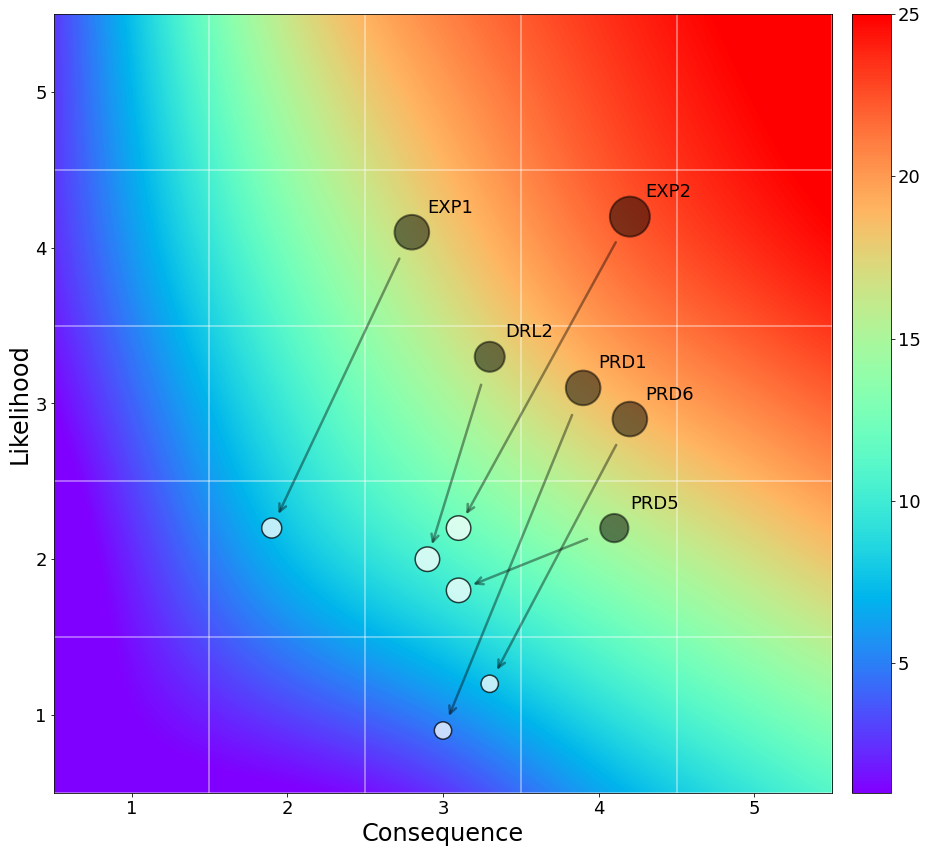
\includegraphics[width=\linewidth]{templates/images/Figure-Risk_Matrix.png}
\caption[Risk matrix]{Risk matrix for categorizing and prioritizing project risks (dark gray) and charting risk mitigation strategies (white). Marker size corresponds with risk value (likelihood $\times$ consequence). Risk labels match those in Table \ref{tab:full_risk_log}.}
\label{fig:risk_matrix}
\end{figure}




\section{Proposed Strategies}